\documentclass[../ai_in_finance]{subfiles}
\usepackage[margin=1in]{geometry}
\usepackage{tikz}
\usetikzlibrary{positioning}
\usepackage{amsmath}
\usepackage{amssymb}
\usepackage{booktabs}
\usepackage{graphicx}
\usepackage{floatrow}
\usepackage{draftwatermark}

\SetWatermarkText{Wulin.Suo@Queensu.ca}
\SetWatermarkScale{0.8}
\SetWatermarkColor{gray!35}
\SetWatermarkAngle{0}
\SetWatermarkVerCenter{0.955\paperheight}

\usepackage{makeidx}
\makeindex

\begin{document}
\input{\subfix{values/ch21}}

\chapterkey{capstone}
\chapter{Case Studies and Capstone Projects}

Every dataset used so far in this book, Cascade Home\index{Cascade Home \& Garden} \& Garden's satellite-derived car counts, Meridian Fabrication\index{Meridian Fabrication Inc.}'s financial statements, the ten-transaction fraud-scoring sample, was built for one purpose: to make a method's mechanics checkable by hand, free of the mess real data carries. That was the right choice for teaching each method in isolation, but it leaves a gap this closing chapter fills. A real financial dataset, of the kind a data scientist downloads from a public repository such as the UCI Machine Learning Repository or Kaggle\index{UCI Machine Learning Repository}\index{Kaggle}, arrives with undocumented category codes, an imbalanced target, correlated and redundant features, and no guarantee that the model that wins on one metric also wins on every other metric that matters.

This chapter works one such dataset end to end, using only tools this book has already built: feature engineering and a model bake-off spanning linear and tree-based methods, from Chapter~\chnum{ml}; Chapter~\chnum{xai}'s SHAP\index{SHAP} and permutation-importance methods, now run with the actual \texttt{shap} library rather than by hand; a cost-sensitive threshold choice extending Chapter~\chnum{fraud}'s alert economics; and a fairness audit extending Chapter~\chnum{xai}'s synthetic two-group example to real data. One topic is new, calibration\index{calibration}, motivated by Chapter~\chnum{creditrisk}'s caveat that a credit score is meaningful only if the probability underneath it is accurate. The chapter closes with governance considerations and further capstone project ideas for the reader.

Two more advanced analyses go beyond a first pass through the pipeline: a systematic hyperparameter search measuring how much tuning gains over a single reasonable configuration, and an intersectional fairness cut that splits the test population two ways at once and uncovers a clear four-fifths-rule violation that the chapter's single-attribute audit, run first, missed.

The dataset is the \emph{Default of Credit Card Clients} dataset\index{Default of Credit Card Clients dataset}\index{credit card!default data} \parencite{yeh2009comparisons}: 30,000 Taiwanese credit card accounts with 23 raw features and a binary label, default on payment the following month, hosted on the UCI Machine Learning Repository and widely distributed on Kaggle under the same name. Unlike every other dataset in this book, it was not built to illustrate anything, and working through it surfaces problems no fictional dataset would: undocumented category codes that must be cleaned before any model is fit, a real 22.1\% default rate rather than a convenient round number, and, as the fairness audits show, a model that passes a single-attribute fairness check comfortably while failing an intersectional one, although no protected attribute is among its inputs.

The chapter follows the order a data scientist follows on a new dataset. It begins by inspecting the raw data closely enough to find its undocumented quirks (Section~\ref{sec:capstone-data}) and engineering features from raw monthly statements rather than from a clean feature table (Section~\ref{sec:capstone-features}). It then compares several model families on the same held-out data (Section~\ref{sec:capstone-bakeoff}) and checks whether the winner's probabilities can be trusted at face value (Section~\ref{sec:capstone-calibration}). From there it explains that model's behavior with real software (Section~\ref{sec:capstone-explain}), converts its output into a lending decision under an explicit cost assumption (Section~\ref{sec:capstone-threshold}), and audits that decision for fairness, first along one dimension (Section~\ref{sec:capstone-fairness}) and then along two at once (Section~\ref{sec:capstone-intersectional}). A discussion of what deploying the pipeline would require (Section~\ref{sec:capstone-governance}) is followed by a reusable template distilled from it (Section~\ref{sec:capstone-template}) and by further capstone projects to apply the template to (Section~\ref{sec:capstone-projects}). Those end the chapter, and the book, on the note Chapter~\chnum{intro} opened with: these tools are only as trustworthy as the discipline applied in using them.

\section{The Data}

The capstone begins where every real project does: with a dataset that is not what its documentation claims.

\subsection{The Capstone Dataset and Its Imperfections}\index{Default of Credit Card Clients dataset!imperfections}
\label{sec:capstone-data}

The raw dataset records, for each of 30,000 accounts, a credit limit (\texttt{LIMIT\_BAL}), demographic fields (\texttt{SEX}, \texttt{EDUCATION}, \texttt{MARRIAGE}, \texttt{AGE}), six months of repayment status codes (\texttt{PAY\_1} through \texttt{PAY\_6}, where $-1$ indicates payment made duly and a positive integer indicates the number of months a payment is overdue), six months of billed amounts (\texttt{BILL\_AMT1}--\texttt{BILL\_AMT6}), six months of amounts actually paid (\texttt{PAY\_AMT1}--\texttt{PAY\_AMT6}), and the target, default on the following month's payment.

Loading the data surfaces the first imperfection the fictional datasets never had: the data dictionary documents \texttt{EDUCATION} as taking values 1 (graduate school), 2 (university), 3 (high school), or 4 (other), yet the column also contains 14 rows coded 0\index{data cleaning!undocumented category codes}\index{Default of Credit Card Clients dataset!undocumented codes}, 280 rows coded 5, and 51 rows coded 6, none of which the documentation defines. \texttt{MARRIAGE} shows the same pattern: documented as 1 (married), 2 (single), or 3 (other), it also contains 54 rows coded 0.

Neither anomaly is disclosed in the documentation, and a modeler who does not notice them will silently feed a model category codes with no defined meaning. Following standard practice for this well-studied dataset, both sets of undocumented codes are folded into their ``other'' categories\index{data cleaning} (0, 5, and 6 into \texttt{EDUCATION}'s category 4; 0 into \texttt{MARRIAGE}'s category 3) before any modeling, a cleaning step with no equivalent elsewhere in this book because every other dataset was built clean.

The repayment-status columns carry two further quirks of the same kind. First, the raw file has no \texttt{PAY\_1} at all: the most recent month's status column is named \texttt{PAY\_0}, while the billed and paid amounts run from \texttt{BILL\_AMT1} and \texttt{PAY\_AMT1}, so the companion notebook renames \texttt{PAY\_0} to \texttt{PAY\_1} to line the three six-month series up. Second, the dictionary defines the status codes as $-1$ (paid duly) and 1 through 9 (months overdue) only, yet the columns are dominated by two undocumented codes, $-2$ and $0$, which together make up 66.9\% of all monthly status entries and appear at least once for 25{,}939 of the 30{,}000 accounts. They are commonly read as ``no balance to pay'' and ``revolving credit, minimum payment made,'' but nothing in the official documentation says so. This chapter leaves them as they are; since both rank below 1, neither counts as a delinquency in the \texttt{max\_\allowbreak delinquency} feature defined below, which is a modeling decision a reader should notice rather than inherit silently.

Table~\ref{tab:capstone_summary} summarizes four representative raw fields before any cleaning or feature engineering; it is worth inspecting closely, the habit Chapter~\chnum{ml} recommended before fitting any model.

\begin{booktable}[htbp]{Summary statistics for four raw fields (before cleaning)}{tab:capstone_summary}
\begin{tabular}{lrrrrr}
\toprule
Field & Mean & Std.\ dev. & Min & Median & Max \\
\midrule
\texttt{LIMIT\_BAL} (NT\$) & 167{,}484 & 129{,}748 & 10{,}000 & 140{,}000 & 1{,}000{,}000 \\
\texttt{AGE} (years) & 35.5 & 9.2 & 21 & 34 & 79 \\
\texttt{BILL\_AMT1} (NT\$) & 51{,}223 & 73{,}636 & $-165{,}580$ & 22{,}382 & 964{,}511 \\
\texttt{PAY\_AMT1} (NT\$) & 5{,}664 & 16{,}563 & 0 & 2{,}100 & 873{,}552 \\
\bottomrule
\end{tabular}
\end{booktable}

\texttt{BILL\_AMT1}'s negative minimum is another undocumented quirk: a negative billed amount means the account was in credit, having overpaid the previous month, a legitimate state for a revolving credit account but one that a modeler unfamiliar with the data might mistake for a data-entry error and drop or clip without justification. \texttt{PAY\_AMT1}'s heavy right skew, a median of just NT\$2,100 against a mean of NT\$5,664 and a maximum of NT\$873,552, is the kind of distribution Section~\ref{sec:capstone-features}'s ratio features are designed to normalize before they reach a linear model, though the tree-based models of Section~\ref{sec:capstone-bakeoff} are much less sensitive to skew than logistic regression\index{logistic regression}, since a tree splits on a feature's rank order rather than its raw scale.

Two more properties of the raw data matter before any model is fit. The first is the class balance. A 22.1\% default rate is much higher than a typical consumer credit-card portfolio, which more commonly runs in the low single digits: a published research dataset's class balance reflects how and when it was sampled, not the balance another institution's portfolio will show. This data covers a six-month window in 2005, shortly before a Taiwanese consumer-credit crisis, so a model built on it should not be assumed to transfer its absolute predicted probabilities to a different portfolio without recalibration, even if its ranking of riskier against safer accounts transfers reasonably well.

The second property is redundancy. Several raw features are highly correlated by construction: the six \texttt{BILL\_AMT} columns track one account's revolving balance from month to month, so they move together. That matters for Section~\ref{sec:capstone-explain}'s explanations, because an importance score assigned to any one of several correlated features is partly arbitrary when the model can substitute one for another with little effect on its predictions. Chapter~\chnum{ml} raised this issue as multicollinearity in linear regression, and it carries over, in a different technical form, to tree-based models and their explanations.

\subsection{From Raw Fields to Model-Ready Features}
\label{sec:capstone-features}\index{feature engineering}

Chapter~\chnum{ml} introduced feature engineering in the abstract; this section performs it on raw fields for the first time. Five engineered features summarize six months of repayment and billing history in a form a model can use more directly than six separate monthly columns. \texttt{max\_\allowbreak delinquency} is the worst (maximum) repayment-status code across the six months, capturing whether an account was ever seriously overdue even if its latest month looks clean. \texttt{avg\_utilization} is the six-month average of billed amount divided by credit limit, a standard credit-risk signal Chapter~\chnum{creditrisk} introduced but never computed from raw statements. \texttt{total\_bill} and \texttt{total\_paid} are the six-month sums of billed and paid amounts, and \texttt{pay\_to\_bill\_ratio} is their ratio, capturing how much of what an account owed it paid back over the window; it is clipped at 5 to bound the influence of a few accounts with a large payment relative to a near-zero bill. These five, together with 20 of the 23 raw fields, give 25 features. The three raw fields left out are \texttt{SEX}, \texttt{MARRIAGE}, and \texttt{AGE}: taking U.S. fair-lending law as the reference point, as Chapter~\chnum{xai} did, the Equal Credit Opportunity Act and its Regulation B forbid basing a credit decision on sex or marital status\index{Equal Credit Opportunity Act (ECOA)}\index{protected attribute} and allow age only in narrow ways (for instance, as a variable in a demonstrably and statistically sound scoring system that never treats applicants aged 62 or older less favorably), so the cleanest choice is to keep all three out of the model and hold \texttt{SEX} and \texttt{AGE} aside as attributes for the fairness audits of Sections~\ref{sec:capstone-fairness} and~\ref{sec:capstone-intersectional}.

The 30,000 accounts are split 80/20 into a training set\index{train-test split} of 24,000 and a held-out test set of 6,000, stratified by the default label so both sets keep the 22.1\% default rate, with a fixed random seed so that the split, and every result in this chapter, is reproducible from the companion notebook. Every model comparison, calibration check, explanation, threshold choice, and fairness audit below is computed on this held-out test set, never on data a model was fit to. Chapter~\chnum{ml} introduced that discipline as essential to detecting overfitting\index{overfitting}, and it matters more once a real dataset's quirks make it easy to believe a model has learned something it has only memorized.

A real dataset also makes another discipline easy to violate: every engineered feature, \texttt{max\_\allowbreak delinquency} included, is computed from information available when each account's repayment history was recorded, not from anything that depends on knowing whether the account defaulted. Chapter~\chnum{altdata}'s point-in-time discipline applies here in a subtler form: a feature engineered carelessly from a dataset that also contains the outcome, for instance a rolling average that accidentally includes a future month's billing data, can leak the label into the features\index{data leakage!target leakage} and produce a model that looks excellent on a test set drawn from the same leaking dataset yet fails once deployed on new applicants for whom the leak is unavailable. This dataset's structure makes such leakage easy to avoid, since every raw field precedes the single target month, but the habit of checking for it explicitly, rather than assuming a clean-looking dataset has none, is one to carry into Section~\ref{sec:capstone-projects}'s further projects, several of which (Lending Club in particular) are much easier to leak by accident.

\begin{bookfigure}[htbp]{The end-to-end pipeline this chapter works through by hand}{fig:capstone_pipeline}
    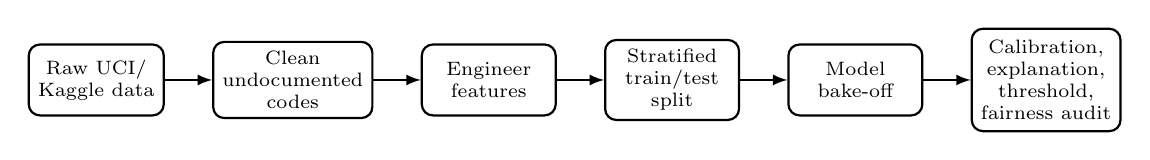
\begin{tikzpicture}[>=latex,thick,node distance=0.6cm]
        \node[draw,rounded corners,minimum width=1.7cm,minimum height=0.9cm,align=center,font=\scriptsize] (raw) {Raw UCI/\\Kaggle data};
        \node[draw,rounded corners,minimum width=1.7cm,minimum height=0.9cm,right=of raw,align=center,font=\scriptsize] (clean) {Clean\\undocumented\\codes};
        \node[draw,rounded corners,minimum width=1.7cm,minimum height=0.9cm,right=of clean,align=center,font=\scriptsize] (feat) {Engineer\\features};
        \node[draw,rounded corners,minimum width=1.7cm,minimum height=0.9cm,right=of feat,align=center,font=\scriptsize] (split) {Stratified\\train/test\\split};
        \node[draw,rounded corners,minimum width=1.7cm,minimum height=0.9cm,right=of split,align=center,font=\scriptsize] (bakeoff) {Model\\bake-off};
        \node[draw,rounded corners,minimum width=1.7cm,minimum height=1.3cm,right=of bakeoff,align=center,font=\scriptsize] (audit) {Calibration,\\explanation,\\threshold,\\fairness audit};
        \draw[->] (raw) -- (clean);
        \draw[->] (clean) -- (feat);
        \draw[->] (feat) -- (split);
        \draw[->] (split) -- (bakeoff);
        \draw[->] (bakeoff) -- (audit);
    \end{tikzpicture}
\end{bookfigure}

\section{Modeling and Evaluation}

This part runs a full bake-off, then asks the questions that decide whether any of it is usable.

\subsection{A Model Bake-Off: Logistic Regression, Random Forests, and Gradient Boosting}
\label{sec:capstone-bakeoff}\index{model bake-off}

Four models are fit on the training set and evaluated, once, on the untouched test set: a plain logistic regression (Chapter~\chnum{ml}'s workhorse, standardized features, no adjustment for class imbalance\index{class imbalance}), a class-weighted logistic regression\index{class imbalance!class weighting} (Chapter~\chnum{fraud}'s first remedy for imbalanced classification, applied here directly rather than to a stylized example), a random forest\index{random forest} (300 trees, Chapter~\chnum{ml}'s bagging-based ensemble), and gradient-boosted trees via XGBoost\index{XGBoost} (300 boosting rounds, Chapter~\chnum{ml}'s sequential, bias-reducing ensemble family, named but not fit by hand in earlier chapters).

Table~\ref{tab:capstone_bakeoff} reports seven metrics for each.

\begin{booktable}[htbp]{Held-out test set performance for four models on the credit-default dataset}{tab:capstone_bakeoff}
\begin{tabular}{lrrrrrrr}
\toprule
Model & Accuracy & Precision & Recall & $F_1$ & ROC-AUC & PR-AUC & Brier \\
\midrule
Logistic (plain) & \vChTwentyOneBakeLRPlainAcc{} & \vChTwentyOneBakeLRPlainPrec{} & \vChTwentyOneBakeLRPlainRec{} & \vChTwentyOneBakeLRPlainFone{} & \vChTwentyOneBakeLRPlainROCAUC{} & \vChTwentyOneBakeLRPlainPRAUC{} & \vChTwentyOneBakeLRPlainBrier{} \\
Logistic (balanced) & \vChTwentyOneBakeLRBalAcc{} & \vChTwentyOneBakeLRBalPrec{} & \vChTwentyOneBakeLRBalRec{} & \vChTwentyOneBakeLRBalFone{} & \vChTwentyOneBakeLRBalROCAUC{} & \vChTwentyOneBakeLRBalPRAUC{} & \vChTwentyOneBakeLRBalBrier{} \\
Random Forest & \vChTwentyOneBakeRFAcc{} & \vChTwentyOneBakeRFPrec{} & \vChTwentyOneBakeRFRec{} & \vChTwentyOneBakeRFFone{} & \vChTwentyOneBakeRFROCAUC{} & \vChTwentyOneBakeRFPRAUC{} & \vChTwentyOneBakeRFBrier{} \\
XGBoost & \vChTwentyOneBakeXGBAcc{} & \vChTwentyOneBakeXGBPrec{} & \vChTwentyOneBakeXGBRec{} & \vChTwentyOneBakeXGBFone{} & \vChTwentyOneBakeXGBROCAUC{} & \vChTwentyOneBakeXGBPRAUC{} & \vChTwentyOneBakeXGBBrier{} \\
\bottomrule
\end{tabular}
\end{booktable}

The plain logistic regression's accuracy (\vChTwentyOneBakeLRPlainAccPct\%) looks respectable in isolation, the trap Chapter~\chnum{fraud} warned against for a rare-event problem\index{class imbalance!evaluation under}: with a 22.1\% default rate, a model far too conservative about flagging defaults can still post high accuracy by predicting the majority class, and this model's recall of only \vChTwentyOneBakeLRPlainRecPct\% shows it misses more than three-quarters of the accounts that default at the standard 0.5 threshold. Class weighting flips the trade-off as Chapter~\chnum{fraud} described: recall rises to \vChTwentyOneBakeLRBalRecPct\% while precision falls from \vChTwentyOneBakeLRPlainPrecPct\% to \vChTwentyOneBakeLRBalPrecPct\%, a much better $F_1$ (\vChTwentyOneBakeLRBalFone{} versus \vChTwentyOneBakeLRPlainFone) but a distinctly worse Brier score\index{Brier score} (\vChTwentyOneBakeLRBalBrier{} versus \vChTwentyOneBakeLRPlainBrier). That pairing is the book's first concrete evidence that class weighting is not a free improvement: reweighting the training loss to counter imbalance also pulls the model's output away from a well-calibrated probability, a cost Chapter~\chnum{fraud} never quantified with a metric like the Brier score, since its worked example used a balanced confusion-matrix illustration rather than a held-out calibration check.

The two tree ensembles dominate both discrimination metrics, ROC-AUC and PR-AUC\index{receiver operating characteristic (ROC) curve}\index{area under the curve (AUC)!ROC-AUC}\index{area under the curve (AUC)!PR-AUC}, over either logistic regression. The comparison also gives Chapter~\chnum{ml}'s bagging-versus-boosting distinction\index{ensemble methods!bagging}\index{ensemble methods!boosting} its first empirical instance: XGBoost's sequential, error-correcting boosting edges out the random forest's parallel, variance-reducing bagging on every metric in the table, though by a narrower margin (ROC-AUC \vChTwentyOneBakeXGBROCAUC{} versus \vChTwentyOneBakeRFROCAUC) than the gap either ensemble opens over logistic regression. That pattern matches a finding well documented in applied machine learning: gradient boosting\index{gradient boosting} and random forests are far closer competitors with each other on tabular data than either is with a linear model, though boosting often comes out slightly ahead.

The comparison also corrects a common oversimplification, that a logistic regression is always the ``safe, interpretable'' choice and a tree ensemble the ``powerful, opaque'' one. Both ensembles beat both logistic regressions on every ranking-based metric by roughly five to six points of ROC-AUC while remaining explainable in Chapter~\chnum{xai}'s sense, with the tooling Section~\ref{sec:capstone-explain} applies below, though not in the coefficient-reading sense that made Chapter~\chnum{creditrisk}'s linear credit-scoring model interpretable by construction.

A lender choosing among these four models is therefore not trading accuracy for interpretability along a single dial; it is trading a small amount of post-hoc explanation overhead (Section~\ref{sec:capstone-explain}'s SHAP computation) for a measurable gain in discrimination and, as Section~\ref{sec:capstone-calibration} shows next, calibration.

\subsection{Is the Model's Probability Actually a Probability? Calibration in Practice}
\label{sec:capstone-calibration}\index{calibration!of probabilities}

Chapter~\chnum{creditrisk} noted that a credit score is meaningful only to the extent that the default probability underneath it is well calibrated, not merely useful for ranking applicants from safest to riskiest; this section makes that check concrete.

\textbf{Calibration} asks whether, among all accounts a model assigns a predicted default probability of, say, 30\%, roughly 30\% actually default. Table~\ref{tab:capstone_calibration} bins the test set into ten deciles of predicted probability\index{calibration!reliability diagram}\index{reliability diagram} for the plain logistic regression and for XGBoost, and compares each decile's average predicted probability to its actual observed default rate.

\begin{booktable}[htbp]{Calibration by predicted-probability decile: plain logistic regression versus XGBoost}{tab:capstone_calibration}
\small
\begin{tabular}{lrrrrr}
\toprule
& \multicolumn{2}{c}{Logistic (plain)} & & \multicolumn{2}{c}{XGBoost} \\
\cmidrule{2-3} \cmidrule{5-6}
Decile (low to high) & Mean predicted & Mean actual & & Mean predicted & Mean actual \\
\midrule
1 & \vChTwentyOneCalLRPredA{} & \vChTwentyOneCalLRActA{} & & \vChTwentyOneCalXGBPredA{} & \vChTwentyOneCalXGBActA{} \\
5 & \vChTwentyOneCalLRPredE{} & \vChTwentyOneCalLRActE{} & & \vChTwentyOneCalXGBPredE{} & \vChTwentyOneCalXGBActE{} \\
6 & \vChTwentyOneCalLRPredF{} & \vChTwentyOneCalLRActF{} & & \vChTwentyOneCalXGBPredF{} & \vChTwentyOneCalXGBActF{} \\
10 & \vChTwentyOneCalLRPredJ{} & \vChTwentyOneCalLRActJ{} & & \vChTwentyOneCalXGBPredJ{} & \vChTwentyOneCalXGBActJ{} \\
\bottomrule
\end{tabular}
\end{booktable}

XGBoost's predicted and actual rates stay within three percentage points of each other in every decile shown (and, in the companion notebook's full table, in every decile not shown), consistent with its lower Brier score in Table~\ref{tab:capstone_bakeoff}. The plain logistic regression shows a visible gap in its lowest decile, an average predicted probability of \vChTwentyOneCalLRPredAPct\% against an actual default rate of \vChTwentyOneCalLRActAPct\%, more than three times higher: the safest-looking accounts by this model's own ranking are much riskier than its probabilities suggest, a miscalibration a lender relying on the raw probability, not just the ranking, would want caught before deployment.

Figure~\ref{fig:capstone_reliability} draws all ten deciles of both models as a \textbf{reliability diagram}\index{calibration!reliability diagram}, together with the isotonic recalibration of the next subsection. Unlike every other figure in this book except those of Chapters~\chnum{python} and~\chnum{valuation}, it and the two that follow are the companion notebook's own matplotlib output rather than redrawn diagrams, because on real data the scatter of the points is itself the evidence. A perfectly calibrated model lies on the diagonal. XGBoost's points hug it from the safest decile to the riskiest. The plain logistic regression's zigzag across it at the low end, where its four lowest deciles predict between $\vChTwentyOneCalLRPredAPct\%$ and $\vChTwentyOneCalLRPredDPct\%$ while the observed default rates jump between $\vChTwentyOneCalLRActLowFourMinPct\%$ and $\vChTwentyOneCalLRActLowFourMaxPct\%$, sag below it through the middle deciles, and finish well above it in the top decile, $\vChTwentyOneCalLRPredJPct\%$ predicted against $\vChTwentyOneCalLRActJPct\%$ observed.

\begin{bookfigure}[htbp][Reliability diagram on the 6,000-account test set]{Reliability diagram on the 6,000-account test set: mean predicted default probability against observed default rate, by decile of each model's own predictions. The recalibrated logistic regression has nine bins because many of its scores tie.}{fig:capstone_reliability}
    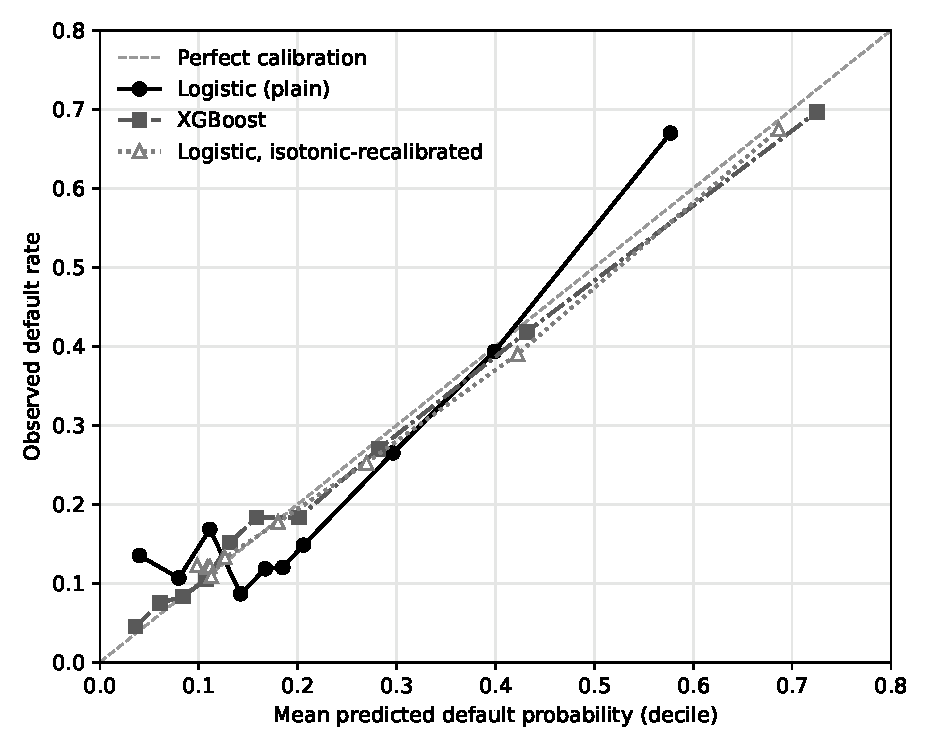
\includegraphics[width=0.72\linewidth]{ch21_fig_reliability.pdf}
\end{bookfigure}

This is why Section~\ref{sec:capstone-threshold}'s cost-sensitive threshold and Section~\ref{sec:capstone-fairness}'s fairness audit both use XGBoost's probabilities rather than the plain logistic regression's: both depend on the predicted probability meaning what it claims, not merely on the model's ability to rank risky accounts above safe ones.

\subsection{Fixing Miscalibration: Isotonic Recalibration}\index{isotonic recalibration}
\label{sec:capstone-isotonic}

The plain logistic regression's calibration gap raises the next question: can it be corrected without discarding the model? \textbf{Isotonic recalibration} fits a separate\index{calibration!isotonic recalibration}, nonparametric, monotonically increasing function that remaps a model's raw probabilities onto better-calibrated ones. The remapping is learned from the data the original model was fit on, but evaluated out-of-fold, Section~\ref{sec:capstone-features}'s train/test discipline applied one level deeper, to the recalibration step itself. Fitting the remapping directly on the test set, as a careless analyst might, would leak the very data the recalibration is meant to be validated against.

Applied to the plain logistic regression, scikit-learn's \texttt{CalibratedClassifierCV}\index{scikit-learn} with isotonic regression, five-fold cross-validated entirely within the training set\index{cross-validation!k-fold}, improves the test-set Brier score from $\vChTwentyOneIsoBrierPlain$ to $\vChTwentyOneIsoBrierCalib$, a modest but real reduction, while leaving ROC-AUC essentially unchanged ($\vChTwentyOneIsoAUCPlain$ before, $\vChTwentyOneIsoAUCCalib$ after). That is what an isotonic remapping should do: because the transformation is monotonic, it cannot change how the model ranks any two applicants, only how well its stated probability matches reality at a given rank. The improvement is concentrated where Table~\ref{tab:capstone_calibration} found the problem.

Recomputing the reliability table on the recalibrated probabilities for the lowest-probability bin,
\begin{align*}
\text{Recalibrated:} &\quad \text{predicted} = \vChTwentyOneIsoLowPredPct\%, \ \text{actual} = \vChTwentyOneIsoLowActPct\%, \ \text{ratio} \approx 1.2, \\
\text{Original (uncalibrated):} &\quad \text{predicted} = \vChTwentyOneCalLRPredAPct\%, \ \text{actual} = \vChTwentyOneCalLRActAPct\%, \ \text{ratio} > 3,
\end{align*} The lesson is general: a model with good discriminative power but poor calibration, the plain logistic regression's situation here, need not be replaced to become a trustworthy probability estimate, only recalibrated, a much cheaper fix than retraining a different model family, and one that leaves all the original coefficients, and so the model's adverse-action interpretability, intact.

Recalibration does not fix everything: XGBoost's Brier score ($\vChTwentyOneBakeXGBBrier$) remains lower than the recalibrated logistic regression's ($\vChTwentyOneIsoBrierCalibThree$), since XGBoost's advantage was never only a calibration artifact. Its higher ROC-AUC in Table~\ref{tab:capstone_bakeoff} reflects superior discriminative power that no monotonic remapping can extract from a linear model's more limited functional form.

Calibration matters beyond this chapter's threshold and fairness exercises. A bank reporting expected credit losses under IFRS 9\index{IFRS 9} or the analogous U.S. CECL\index{Current Expected Credit Losses (CECL)} framework multiplies a probability of default directly into a provisioning calculation\index{provisioning}, Chapter~\chnum{creditrisk}'s $\text{EL} = \text{PD} \times \text{LGD} \times \text{EAD}$ decomposition. A systematically miscalibrated probability, not merely a poorly ranked one, therefore becomes an over- or understated loss provision in the bank's financial statements, the kind of number Chapter~\chnum{statements} taught how to read and Chapter~\chnum{creditrisk} how to model, and one that depends on a property, calibration, that neither accuracy nor ROC-AUC guarantees.

Section~\ref{sec:capstone-explain} returns to this formula with real provisioning numbers, once this chapter's own low-risk and high-risk applicants have been introduced.

\subsection{Explaining a Real, Nonlinear Model: SHAP and Permutation Importance}
\label{sec:capstone-explain}\index{explainability}

Chapter~\chnum{xai} computed an exact Shapley decomposition\index{Shapley value} by hand for Chapter~\chnum{creditrisk}'s credit-scoring model only because that model was linear in the log-odds; XGBoost is not. The \texttt{shap} library's \texttt{TreeExplainer}\index{SHAP!TreeExplainer}\index{TreeExplainer} algorithm computes exact Shapley values efficiently for tree ensembles by exploiting the tree structure directly, rather than relying on the linear shortcut or on sampled perturbations as Chapter~\chnum{xai}'s LIME\index{LIME (Local Interpretable Model-agnostic Explanations)} example did.

Table~\ref{tab:capstone_importance} compares the resulting global feature ranking, mean absolute SHAP value across 1,000 held-out accounts, against Chapter~\chnum{xai}'s other global method, permutation importance\index{permutation feature importance} (here, the drop in ROC-AUC when a feature is shuffled), computed on the full test set.

\begin{booktable}[htbp]{Top features by two global importance methods, XGBoost model}{tab:capstone_importance}
\begin{tabular}{lrlr}
\toprule
Rank & Permutation importance (feature) & & Mean $|\text{SHAP}|$ (feature) \\
\midrule
1 & \texttt{PAY\_1} (\vChTwentyOnePermA) & & \texttt{max\_\allowbreak delinquency} (\vChTwentyOneShapA) \\
2 & \texttt{max\_\allowbreak delinquency} (\vChTwentyOnePermB) & & \texttt{PAY\_1} (\vChTwentyOneShapB) \\
3 & \texttt{avg\_utilization} (\vChTwentyOnePermC) & & \texttt{avg\_utilization} (\vChTwentyOneShapC) \\
4 & \texttt{BILL\_AMT1} (\vChTwentyOnePermD) & & \texttt{BILL\_AMT1} (\vChTwentyOneShapD) \\
5 & \texttt{LIMIT\_BAL} (\vChTwentyOnePermE) & & \texttt{LIMIT\_BAL} (\vChTwentyOneShapE) \\
\bottomrule
\end{tabular}
\end{booktable}

The two methods agree on which five features matter (the most recent repayment status, the worst repayment status over six months, utilization, the most recent bill, and credit limit) and order ranks three through five identically, but disagree on the top two: permutation importance ranks the most recent month's repayment status (\texttt{PAY\_1}) above the worst status across six months, while SHAP ranks them the other way around. Neither ranking is wrong; they answer different questions, as Chapter~\chnum{xai} cautioned: permutation importance describes a feature's contribution to a specific performance metric on specific data, while SHAP describes each feature's average marginal contribution to individual predictions. A modeler who reports only one of the two risks a false precision about which single feature ``matters most.''

A single applicant's explanation shows at the individual level\index{local explanation} what Section~\ref{sec:capstone-bakeoff}'s aggregate table cannot. The first test-set applicant is assigned a predicted default probability of $\vChTwentyOneLowPDPct\%$ by XGBoost.

SHAP's additive decomposition operates on the model's raw log-odds output rather than on the probability, as Chapter~\chnum{xai}'s exact Shapley decomposition did for the linear credit-scoring model. This applicant's base value, the average log-odds prediction across the training population, is $\vChTwentyOneShapBase$, and summing the SHAP contributions of every feature gives a total log-odds of $\vChTwentyOneLowLogOdds$. The sigmoid converts that back to $\vChTwentyOneLowPDPct\%$, matching the model's output: the completeness property Chapter~\chnum{xai} checked by hand for a linear model, now confirmed for a nonlinear ensemble. The applicant's largest contributions are
\begin{align*}
\texttt{max\_\allowbreak delinquency} = 0 \text{ (no serious delinquency):} &\quad \text{SHAP} = \vChTwentyOneLowShapA, \\
\texttt{avg\_utilization} = 12.1\% \text{ (low):} &\quad \text{SHAP} = \vChTwentyOneLowShapB, \\
\text{Credit limit} = \text{NT}\$50{,}000 \text{ (modest):} &\quad \text{SHAP} = \vChTwentyOneLowShapC, \\
\text{Most-recent repayment status} = -1 \text{ (paid duly):} &\quad \text{SHAP} = \vChTwentyOneLowShapD,
\end{align*}
the modest credit limit contributing positively to predicted risk since, in this dataset, lower limits are associated with higher-risk accounts.

Figure~\ref{fig:capstone_waterfall} draws the whole decomposition as a \textbf{waterfall}\index{SHAP!waterfall plot}: starting from the base value of $\vChTwentyOneShapBase$, each bar moves the running log-odds by one feature's SHAP value, hatched bars raising predicted risk and plain bars lowering it. The seven largest contributions are shown individually; the remaining 18 features together contribute $\vChTwentyOneLowShapRest$, and the bars end at $\vChTwentyOneLowLogOdds$, the model's actual output, which is the completeness property made visible.

\begin{bookfigure}[htbp][SHAP waterfall for the low-risk applicant]{SHAP waterfall for the low-risk applicant (predicted default probability $\vChTwentyOneLowPDPct\%$), in log-odds. Hatched bars increase predicted risk; plain bars decrease it. The dashed line marks the base value and the solid line the model's output.}{fig:capstone_waterfall}
    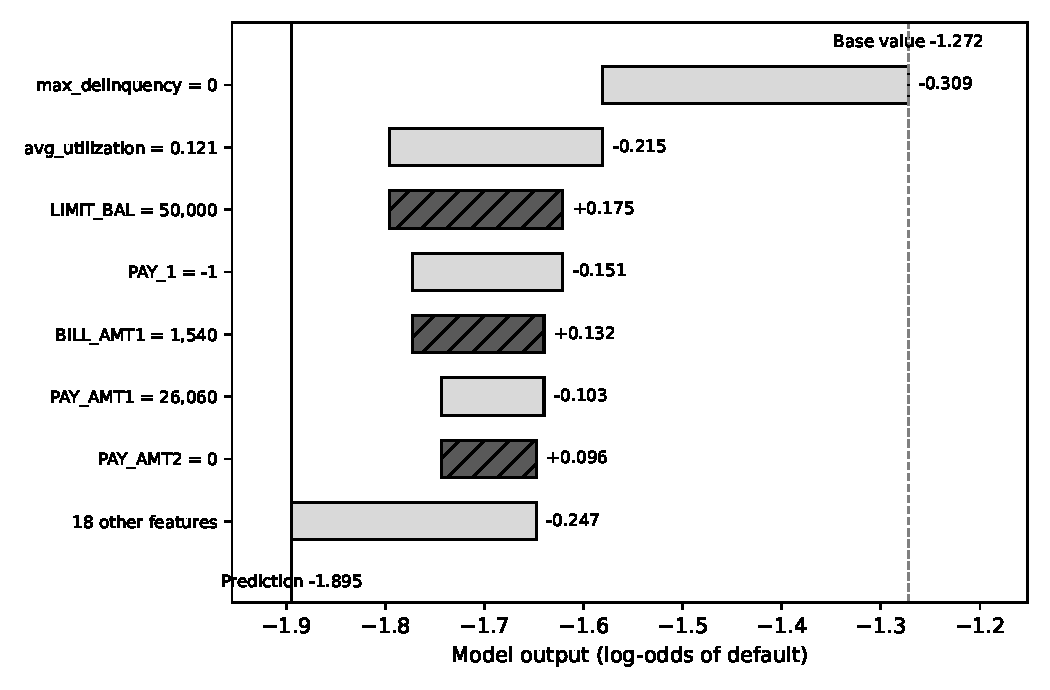
\includegraphics[width=0.78\linewidth]{ch21_fig_shap_waterfall.pdf}
\end{bookfigure}

Chapter~\chnum{xai}'s adverse-action reason codes followed automatically from a linear model's coefficients; for a deployed ensemble, producing the same kind of individualized explanation requires this extra step, running \texttt{TreeExplainer} against the fitted model, before a bank can issue a model-derived reason to an applicant under the Equal Credit Opportunity Act\index{Equal Credit Opportunity Act (ECOA)}.

A contrasting high-risk applicant\index{SHAP!low-risk versus high-risk applicants} from the same test sample makes the method's value clearer. This applicant is assigned a predicted default probability of $\vChTwentyOneHighPDPct\%$, and the same decomposition gives a base value of $\vChTwentyOneShapBase$ and a summed log-odds of $\vChTwentyOneHighLogOdds$ (whose sigmoid is, again exactly, $\vChTwentyOneHighPDPct\%$). Here the dominant contributions run the other way:
\begin{align*}
\text{Most-recent repayment status} = 3 \text{ (three months overdue):} &\quad \text{SHAP} = \vChTwentyOneHighShapA, \\
\text{Worst-ever repayment status} = 7 \text{ (severely delinquent):} &\quad \text{SHAP} = \vChTwentyOneHighShapB, \\
\text{Credit limit} = \text{NT}\$10{,}000 \text{ (the dataset's minimum):} &\quad \text{SHAP} = \vChTwentyOneHighShapC,
\end{align*}
with \texttt{pay\_to\_bill\_ratio} $= 0$ (repaid essentially nothing over six months) adding a further $\vChTwentyOneHighShapF$, and the most-recent-repayment contribution the single largest seen in either applicant's decomposition.

Side by side, the two explanations read almost as mirror images: no delinquency history and full repayment push one applicant's risk sharply down, while recent, severe delinquency and near-zero repayment push the other's sharply up. That individualized contrast is what an adverse-action notice or a credit-committee review needs, and what an aggregate importance ranking like Table~\ref{tab:capstone_importance} cannot provide.

\weheading{\subsubsection*}{capstone-provisioning}{From Predicted Probability to a Provisioning Number}\index{expected loss!PD, LGD, EAD}

Section~\ref{sec:capstone-calibration} promised to return to Chapter~\chnum{creditrisk}'s $\text{EL} = \text{PD} \times \text{LGD} \times \text{EAD}$ decomposition with real numbers; the two applicants supply them. Each applicant's credit limit stands in for exposure at default\index{exposure at default (EAD)}, a standard simplification for a revolving line assumed fully drawn at default, and, with no collateral information for an unsecured card balance, the example reuses Chapter~\chnum{creditrisk}'s illustrative\index{loss given default (LGD)} $\text{LGD}=60\%$.

All amounts in this dataset are in New Taiwan dollars (NT\$), not U.S. dollars; at the 2005 exchange rate of roughly NT\$32 to the U.S. dollar, the low-risk applicant's NT\$50{,}000 limit is worth only about US\$1{,}550. For the low-risk applicant, $\text{PD}=\vChTwentyOneLowPDPctFive\%$ (the $\vChTwentyOneLowPDPct\%$ reported earlier, carried to more decimals to reproduce the figure below exactly by hand) and $\text{EAD}=\text{NT}\$50{,}000$ (this applicant's \texttt{LIMIT\_BAL}), giving
\begin{equation*}
\text{EL}_{\text{low-risk}} = \vChTwentyOneLowPDSeven{} \times 0.60 \times \text{NT}\$50{,}000 = \text{NT}\$\vChTwentyOneELLow,
\end{equation*}
while the high-risk applicant, with $\text{PD}=\vChTwentyOneHighPDPctFive\%$ (similarly carried to more decimals) and a much smaller $\text{EAD}=\text{NT}\$10{,}000$ (a lower credit limit, itself consistent with this applicant's weaker profile), gives
\begin{equation*}
\text{EL}_{\text{high-risk}} = \vChTwentyOneHighPDSeven{} \times 0.60 \times \text{NT}\$10{,}000 = \text{NT}\$\vChTwentyOneELHigh.
\end{equation*}

The high-risk applicant's expected loss is only about $\vChTwentyOneELRatio\times$ the low-risk applicant's, a far smaller multiple than the $\vChTwentyOnePDRatio\times$ gap in predicted default probability ($\vChTwentyOneHighPDPctTwo\%/\vChTwentyOneLowPDPct\%$), because the high-risk applicant's credit limit, one-fifth of the other's, largely offsets the higher probability: an interaction among the three inputs to expected loss that looking at PD alone would miss. A bank provisioning against its whole card portfolio sums a version of this calculation across every account, so a systematic miscalibration of the kind Section~\ref{sec:capstone-calibration} found in the plain logistic regression, understating risk in the lowest-probability decile, would understate provisions for the bank's safest-looking accounts, the segment a supervisor examining provisioning adequacy would be least likely to scrutinize.

\texttt{TreeExplainer} is also fast: it computes exact Shapley values for a tree ensemble in time roughly proportional to the number of trees times the square of tree depth, rather than the exponential cost of the general, model-agnostic Shapley formula Chapter~\chnum{xai} mentioned, which is why it can run here against a several-hundred-tree ensemble rather than only against the small linear toy models of Chapter~\chnum{xai}'s hand computations. This matters operationally: a bank issuing thousands of adverse-action notices a month needs an explanation method fast enough for that volume, and a sampling-based method like LIME, useful for a single illustrative explanation, does not scale as cleanly as an algorithm built for the model family being explained.

\subsection{Choosing an Operating Threshold: A Real Cost-Sensitive Analysis}
\label{sec:capstone-threshold}\index{cost-sensitive threshold}\index{decision threshold!cost-sensitive choice}

Every result so far used the default 0.5 threshold. Chapter~\chnum{fraud}'s alert-economics section argued that the right threshold is a business decision balancing the cost of a missed default against the cost of denying a good customer, not a property of the model, and this section quantifies that trade-off. Assigning an illustrative cost of \$500 to a missed default (a false negative, an account that defaults but is approved) and \$50 to wrongly denying a good customer (a false positive, a tenth of the missed-default cost, since a denied good customer typically costs foregone interest rather than lost principal), the expected total cost across the test set at threshold $t$ is $\text{Cost}(t) = 500 \cdot FN(t) + 50 \cdot FP(t)$.

Table~\ref{tab:capstone_threshold} sweeps this across a grid of thresholds using XGBoost's predicted probabilities.

\begin{booktable}[htbp]{Cost-sensitive threshold sweep, XGBoost model, held-out test set}{tab:capstone_threshold}
\begin{tabular}{lrrr}
\toprule
Threshold & False negatives & False positives & Total cost \\
\midrule
0.05 & \vChTwentyOneCostAFN{} & \vChTwentyOneCostAFP{} & \$\vChTwentyOneCostATotal{} \\
0.10 (cost-minimizing) & \vChTwentyOneCostBFN{} & \vChTwentyOneCostBFP{} & \$\vChTwentyOneCostBTotal{} \\
0.20 & \vChTwentyOneCostCFN{} & \vChTwentyOneCostCFP{} & \$\vChTwentyOneCostCTotal{} \\
0.35 & \vChTwentyOneCostDFN{} & \vChTwentyOneCostDFP{} & \$\vChTwentyOneCostDTotal{} \\
0.50 (naive default) & \vChTwentyOneCostEFN{} & \vChTwentyOneCostEFP{} & \$\vChTwentyOneCostETotal{} \\
0.60 & \vChTwentyOneCostFFN{} & \vChTwentyOneCostFFP{} & \$\vChTwentyOneCostFTotal{} \\
\bottomrule
\end{tabular}
\end{booktable}

The cost-minimizing threshold on this grid is $t = 0.10$, far below the naive 0.5 default, at a total expected cost of \$\vChTwentyOneCostBTotalComma, versus \$\vChTwentyOneCostETotalComma{} at the naive threshold, more than double. That value could have been predicted without a sweep. Denying an account with predicted default probability $p$ is cheaper than approving it whenever $p \times \$500 > (1-p) \times \$50$, so for a calibrated model the cost-minimizing threshold is
\begin{equation}
t^{*} = \frac{c_{FP}}{c_{FP} + c_{FN}} = \frac{50}{50 + 500} = 0.091,
\label{eq:capstone-threshold}
\end{equation}
the same expected-cost comparison Chapter~\chnum{fraud} used to derive its fraud-review threshold, adapted to a decision in which a correctly denied defaulter costs nothing. Only the ratio of the two costs matters, not their level or currency. The grid's empirical minimum at $0.10$ sits right next to this analytic value (at exactly $0.091$ the test-set cost is \$\vChTwentyOneCostAtTStarComma, the small difference being sampling noise in 6,000 accounts), a further check on Section~\ref{sec:capstone-calibration}'s finding that XGBoost's probabilities are well calibrated.

Figure~\ref{fig:capstone_cost_curve} plots the cost at every threshold on the $0.01$-spaced grid behind Table~\ref{tab:capstone_threshold}. Its shape carries a practical message the table only hints at: the curve is nearly flat around its minimum, from \$\vChTwentyOneCostATotal{} at $t=0.05$ to \$\vChTwentyOneCostBTotal{} at $t=0.10$, and then climbs steeply and almost linearly toward \$\vChTwentyOneCostETotal{} at the naive threshold. Setting the threshold somewhat too low is cheap here; setting it far too high is expensive.

\begin{bookfigure}[htbp][Total expected cost against the classification threshold, XGBoost model]{Total expected cost on the test set, $500\,FN(t) + 50\,FP(t)$, against the classification threshold $t$, XGBoost model. The solid vertical line marks the grid minimum at $t=0.10$, the dotted line the analytic threshold $t^{*}=0.091$, and the dashed line the naive $t=0.5$.}{fig:capstone_cost_curve}
    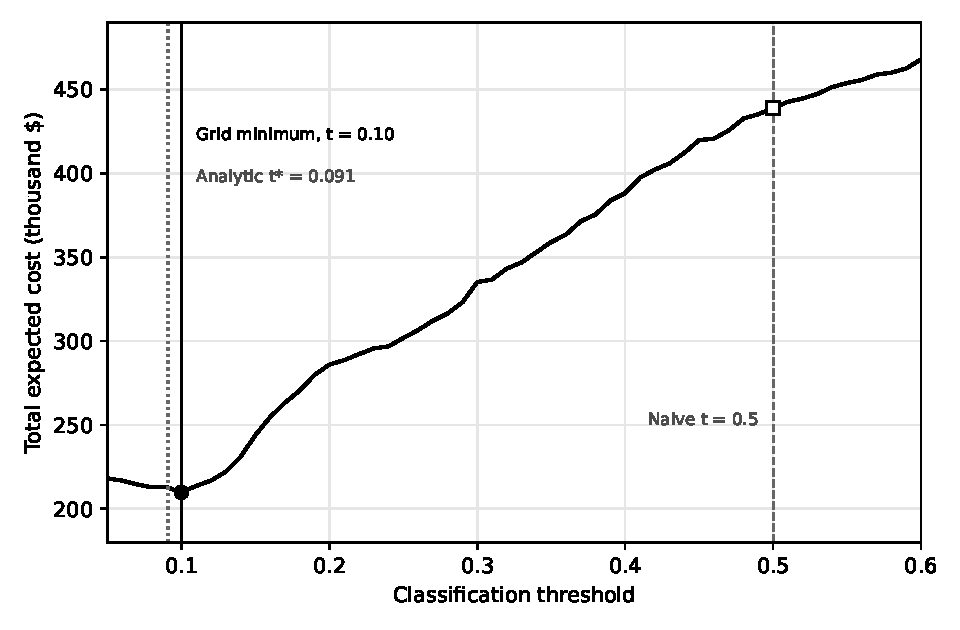
\includegraphics[width=0.75\linewidth]{ch21_fig_cost_threshold.pdf}
\end{bookfigure}

The gap between \$209,750 and \$438,900 is the lesson: choosing a threshold by convention rather than by the institution's cost structure leaves real money on the table, much more here than the gap between any two models in Table~\ref{tab:capstone_bakeoff}, which is why Chapter~\chnum{fraud} treated threshold choice as at least as consequential as model choice. The optimal threshold depends entirely on the assumed 10-to-1 cost ratio; a lender who judged missed defaults and denied good customers comparably costly would land much closer to 0.5. This is a business judgment, not a number the chapter's methods can supply.

The resulting operating point deserves a plain statement: at $t = 0.10$ the model approves only \vChTwentyOneApproveBestPct\% of the test accounts, against \vChTwentyOneApproveNaivePct\% at the naive 0.5 threshold, and turns away \vChTwentyOneGoodDeniedPct\% of the accounts that would not have defaulted. No real card lender operates anywhere near so strict a cutoff. The toy cost ratio drives it: charging a missed default only ten times a wrongly denied good customer, against a 22.1\% base default rate, pushes the threshold below the probability most accounts are assigned. A real lender's cost of denying a good customer includes the lifetime value of the relationship, and the cost of a missed default is proportional to the exposure rather than flat, so a realistic cost model would place the threshold, and the approval rate, very differently.

The threshold sweep is a cost-weighted walk along the receiver operating characteristic curve\index{receiver operating characteristic (ROC) curve} Chapter~\chnum{ml} introduced. Each threshold in Table~\ref{tab:capstone_threshold} is one point on that curve, trading fewer false negatives for more false positives as the threshold falls. What this section adds is not a new statistical concept but a conversion of that trade-off into dollars, so the operating point is chosen by comparing two cost figures rather than by picking a point on a curve that looks like a reasonable compromise.

A lender would also stress-test this choice, as Chapter~\chnum{creditrisk} stress-tested a credit portfolio: if a recession doubled the cost of a missed default relative to a denied applicant, the cost-minimizing threshold would fall further, flagging more accounts as high-risk, the scenario analysis a model-risk function should run before committing to a single operating threshold in production.

\subsection{A Real Fairness Audit}
\label{sec:capstone-fairness}\index{fairness audit}

Chapter~\chnum{xai}'s fairness audit used a synthetic eight-applicant dataset built to make a point cleanly; this section runs the same audit, the four-fifths rule\index{four-fifths rule} and an error-rate comparison, on the real test set at the cost-minimizing threshold of Section~\ref{sec:capstone-threshold}, split by the dataset's \texttt{SEX} field. Table~\ref{tab:capstone_fairness} reports the results.

\begin{booktable}[htbp]{A fairness audit by sex, XGBoost model at the cost-minimizing threshold ($t=0.10$)}{tab:capstone_fairness}
\begin{tabular}{lrrrr}
\toprule
Group & $n$ & Approval rate & False-negative rate & False-positive rate \\
\midrule
Male & 2{,}402 & \vChTwentyOneFairMaleApprovePct\% & \vChTwentyOneFairMaleFNRPct\% & \vChTwentyOneFairMaleFPRPct\% \\
Female & 3{,}598 & \vChTwentyOneFairFemaleApprovePct\% & \vChTwentyOneFairFemaleFNRPct\% & \vChTwentyOneFairFemaleFPRPct\% \\
\bottomrule
\end{tabular}
\end{booktable}

The adverse impact ratio\index{adverse impact ratio}, computed from the unrounded approval rates as $\vChTwentyOneFairMaleApprovePctTwo\%/\vChTwentyOneFairFemaleApprovePctTwo\% = \vChTwentyOneFairAIR$, clears the 80\% four-fifths threshold of Chapter~\chnum{xai}'s fairness section by a wide margin, and some gap is expected, since male accounts in the test set default more often (23.4\% against 21.3\%). The error rates show the tension\index{fairness!equalized odds} Chapter~\chnum{xai}'s synthetic example illustrated, now on real data: the group with the higher approval rate (female accounts) also has the higher false-negative rate, missing \vChTwentyOneFairFemaleFNRPct\% of accounts that go on to default, against \vChTwentyOneFairMaleFNRPct\% for male accounts, so the group favored by the headline approval rate is the group whose default risk this threshold captures less completely. Neither comparison is ``the'' fairness result; both are properties of the same model and threshold, and, as Chapter~\chnum{xai}'s impossibility result predicts, no adjustment to this one threshold can bring both gaps to zero unless the groups' underlying default rates coincide.

Leaving the protected attributes out of the model mattered: the same XGBoost configuration refit with \texttt{SEX}, \texttt{MARRIAGE}, and \texttt{AGE} as inputs, which the companion notebook runs for contrast, approves \vChTwentyOneDemoMaleApprovePct\% of male and \vChTwentyOneDemoFemaleApprovePct\% of female accounts at the same threshold, an adverse impact ratio of only \vChTwentyOneDemoAIR, while scoring essentially no better (test ROC-AUC \vChTwentyOneDemoAUC{} against \vChTwentyOneBakeXGBROCAUC). But removing the attributes did not remove the difference. The model never sees \texttt{SEX}, yet its decisions still differ measurably by sex, the pattern of Chapter~\chnum{xai}'s Apple Card\index{Apple Card gender-bias controversy} vignette: ``fairness through unawareness'' narrows a disparity\index{protected attribute}\index{proxy discrimination!lending} only as far as the remaining features fail to encode the omitted attribute. What the audit does not establish is why the residual difference exists: whether it reflects the groups' different default rates or another feature correlated with sex closely enough to reproduce the pattern. Income proxies and credit-limit history are the leading suspects in this dataset, though testing that rigorously would require the counterfactual-fairness framing\index{counterfactual fairness} of Chapter~\chnum{xai}'s advanced topics, not merely this correlational check. Section~\ref{sec:capstone-intersectional} then shows that this single-attribute finding, reassuring as its $\vChTwentyOneFairAIR$ ratio looks, does not remotely tell the whole story once a second characteristic is added.

\section{From Model to Project}

A model is not a project; this part covers deployment, and the template for doing all of it again.

\subsection{From Model to Deployment: Governance Considerations}
\label{sec:capstone-governance}\index{model deployment!governance}\index{AI governance}

Chapter~\chnum{xai}'s governance section organized model governance around SR 11-7\index{SR 11-7}'s three pillars, conceptual soundness, ongoing monitoring, and outcomes analysis, which SR 26-2, the guidance that superseded it\index{SR 26-2} in April 2026, keeps intact \parencite{frb2026revised}, and this pipeline maps onto all three.

Conceptual soundness is Section\index{model validation}~\ref{sec:capstone-bakeoff}'s model bake-off and Section~\ref{sec:capstone-calibration}'s calibration check, documented well enough that an independent validator, Chapter~\chnum{fraud}'s second line of defense, could reproduce every number in Table~\ref{tab:capstone_bakeoff} from the companion notebook without re-deriving the modeling choices. Outcomes analysis is Section~\ref{sec:capstone-fairness}'s fairness audit, which this chapter's numbers show passing on one cut (\vChTwentyOneFairAIR{} by sex) and failing on another (Section~\ref{sec:capstone-intersectional}'s sex-by-age cut), so a one-time check at deployment is not enough; ongoing monitoring, with Chapter\index{model monitoring!population stability index}~\chnum{xai}'s population stability index\index{population stability index (PSI)} on this feature set and a recurring rerun of both audits, is what would catch a shift in the applicant pool moving either ratio before an examiner does.

None of this replaces human judgment: Section~\ref{sec:capstone-threshold}'s cost assumptions, the \$500-to-\$50 ratio driving the threshold, are a business decision no algorithm here can make for the institution, the kind of accountable, documented judgment that Chapter~\chnum{fraud}'s three-lines-of-defense framework and the NIST AI RMF\index{NIST AI Risk Management Framework}'s ``govern'' function exist to make explicit.

A deployment checklist follows\index{model deployment} from the chapter's sections. Before the model scores a real applicant, an institution would need Section~\ref{sec:capstone-data}'s cleaning logic and Section~\ref{sec:capstone-features}'s feature engineering encoded in a reproducible data pipeline\index{reproducibility} rather than a one-off notebook cell. It would need Section~\ref{sec:capstone-bakeoff}'s model selection and Section~\ref{sec:capstone-tuning}'s hyperparameter search documented well enough for a validator to rerun them and obtain the same numbers. It would need Section~\ref{sec:capstone-calibration}'s calibration check and Section~\ref{sec:capstone-threshold}'s cost assumptions re-approved on a recurring basis, since calibration and an institution's true cost ratio both drift as the applicant population and business environment change. And it would need the fairness audits of Sections~\ref{sec:capstone-fairness} and~\ref{sec:capstone-intersectional}, the intersectional cut included, rerun on every new cohort of applicants, because Section~\ref{sec:capstone-intersectional} showed that a single-attribute check passing today is no guarantee that a deeper cut will not fail tomorrow.

\subsection{Advanced Topics}
\label{sec:capstone-advanced}

Two further analyses go beyond a first pass: a systematic search over XGBoost's hyperparameters, to see how much Section~\ref{sec:capstone-bakeoff}'s single configuration left on the table, and a fairness audit that splits the test set two ways at once, revealing a disparity Section~\ref{sec:capstone-fairness}'s single-attribute audit could not see.

\subsection{Hyperparameter Tuning: Diminishing Returns in Practice}
\label{sec:capstone-tuning}\index{hyperparameter tuning!diminishing returns}

Section~\ref{sec:capstone-bakeoff}'s XGBoost model used a single, manually chosen configuration (300 trees, maximum depth 4, learning rate 0.05). A randomized search over 30 candidate configurations\index{hyperparameter tuning} varied tree depth (3 to 6), learning rate (0.01 to 0.1), the number of boosting rounds (100 to 500), the row and column subsampling fractions, and the minimum child weight controlling how conservatively a tree can split. Every candidate was evaluated by five-fold cross-validation\index{cross-validation!k-fold}\index{cross-validation} on the training set alone, never touching the test set: Section~\ref{sec:capstone-features}'s train/test discipline applied one level deeper, since a hyperparameter search must also be validated on data it never saw.

The best configuration found, depth 4, learning rate 0.1, 100 rounds, no row subsampling, 60\% column subsampling, and a minimum child weight of 5, achieved a cross-validated ROC-AUC of $\vChTwentyOneTunedCVAUC$, and, refit on the full training set and evaluated once on the held-out test set, a test ROC-AUC of $\vChTwentyOneTunedAUC$, a PR-AUC of $\vChTwentyOneTunedPRAUC$, and a Brier score of $\vChTwentyOneTunedBrier$. Compared against Section~\ref{sec:capstone-bakeoff}'s untuned XGBoost model (test ROC-AUC $\vChTwentyOneBakeXGBROCAUC$, PR-AUC $\vChTwentyOneBakeXGBPRAUC$, Brier $\vChTwentyOneBakeXGBBrier$), the result of a reasonably thorough search is not even a uniform improvement: ROC-AUC rises by three thousandths, PR-AUC falls by three thousandths, and the Brier score does not move at the third decimal, all changes far smaller than the gap either tree ensemble opened up over logistic regression in Table~\ref{tab:capstone_bakeoff}.

This is a useful, if unexciting, finding. Once a model family is well chosen and its configuration set to sensible, moderate values, as Section~\ref{sec:capstone-bakeoff}'s untuned model already was, further search on a dataset of this size and feature set faces diminishing returns. The gap between the cross-validated score ($\vChTwentyOneTunedCVAUC$) and the held-out test score ($\vChTwentyOneTunedAUC$) is a small reminder that a search's selected score is mildly optimistic, having been chosen among 30 candidates because it performed best on that particular split.

\subsection{Intersectional Fairness: What Aggregation Can Hide}
\label{sec:capstone-intersectional}\index{intersectional fairness}\index{fairness!intersectional}

Section~\ref{sec:capstone-fairness}'s audit split the test set only by sex. Splitting it a second way at the same time, by sex and by an age cutoff at 30 years, reveals a pattern the single-attribute audit could not, shown in Table~\ref{tab:capstone_intersectional}.

\begin{booktable}[htbp]{An intersectional fairness cut: sex crossed with age group}{tab:capstone_intersectional}
\begin{tabular}{llrrr}
\toprule
Sex & Age group & $n$ & Approval rate & False-negative rate \\
\midrule
Male & Under 30 & 669 & \vChTwentyOneInterMaleYoungApprovePct\% & \vChTwentyOneInterMaleYoungFNRPct\% \\
Male & 30 and over & 1{,}733 & \vChTwentyOneInterMaleOlderApprovePct\% & \vChTwentyOneInterMaleOlderFNRPct\% \\
Female & Under 30 & 1{,}243 & \vChTwentyOneInterFemaleYoungApprovePct\% & \vChTwentyOneInterFemaleYoungFNRPct\% \\
Female & 30 and over & 2{,}355 & \vChTwentyOneInterFemaleOlderApprovePct\% & \vChTwentyOneInterFemaleOlderFNRPct\% \\
\bottomrule
\end{tabular}
\end{booktable}

The most disadvantaged subgroup by approval rate, young men under 30, is approved only $\vChTwentyOneInterMaleYoungApprovePct\%$ of the time, against $\vChTwentyOneInterMaleOlderApprovePct\%$ for the most favored subgroup, men 30 and over. That is an adverse impact ratio, from the unrounded rates, of $\vChTwentyOneInterMaleYoungApprovePctTwo\%/\vChTwentyOneInterMaleOlderApprovePctTwo\% = \vChTwentyOneInterAIR$, a clear four-fifths-rule violation, and it stands in sharp contrast\index{four-fifths rule} to Section~\ref{sec:capstone-fairness}'s sex-only audit, which found a ratio of $0.960$, comfortably on the right side of the same threshold. The two findings are not in tension; they answer different questions. Averaging young and older men together in the sex-only audit hides that young men, on their own, face a starkly lower approval rate than any other subgroup, a disparity the single-attribute view cannot see because it never asks. Nor is this simply an age effect that a separate age audit would have caught at the same strength: among women the under-30 group is approved at $\vChTwentyOneInterFemaleYoungApprovePct\%$ against $\vChTwentyOneInterFemaleOlderApprovePct\%$, a ratio of about \vChTwentyOneInterFemaleRatio, so the shortfall is concentrated where the two characteristics meet. It also arises in a model that, as Section~\ref{sec:capstone-features} specified, never sees \texttt{AGE} at all, a second and sharper instance of Section~\ref{sec:capstone-fairness}'s point that leaving an attribute out does not keep the features that correlate with it, shorter credit histories and lower assigned limits among the youngest borrowers, from carrying it back in; the most obvious such feature here is \texttt{LIMIT\_BAL}\index{proxy discrimination!lending}, since the youngest borrowers, and young men above all, hold markedly lower credit limits (a median of NT\$80{,}000 for men under 30 in the test set, against NT\$150{,}000 for men 30 and over). This is the failure mode intersectional or subgroup analysis exists to catch, and that fair-lending examiners and model validators test for: a model can pass every single-attribute audit an institution runs and still produce a stark disparity for a subgroup defined by two or more characteristics, and the only way to find it is to look for it, since Table~\ref{tab:capstone_fairness}'s aggregate numbers give no hint that it exists.

A thorough fairness audit therefore cannot stop at a single-attribute cut, however clean its result; it must cross every combination of characteristics an institution has reason to worry about, a much larger testing burden than a single audit table suggests, and, as this dataset shows, not merely a theoretical one. The 2026 change in U.S. federal law does not remove that burden. Since 21 July 2026 Regulation B no longer carries a disparate-impact\index{Regulation B}\index{disparate impact} ``effects test'' under the Equal Credit Opportunity Act \parencite{cfpb2026regb}, so a ratio below 0.80 is not by itself a federal fair-lending violation; but the four-fifths rule remains the standard screening heuristic, state enforcers and regimes abroad still reach disparate outcomes (Chapter~\chnum{xai}'s table of regulatory regimes), and model-risk governance expects such a disparity to be found and explained either way.

\subsection{A Template for Completing a Capstone Project}
\label{sec:capstone-template}\index{capstone project!nine-stage template}

Section~\ref{sec:capstone-projects} lists several real datasets a reader could build a capstone project on. This section is the template for doing so: a stage-by-stage checklist distilled from this chapter's pipeline (Figure~\ref{fig:capstone_pipeline}), so that a reader starting from any dataset on that list, or one of their own, has a concrete standard to work toward rather than an open-ended instruction to ``build a model.'' Each stage in Table~\ref{tab:capstone_template} names the tool this chapter or an earlier one developed for it, along with a deliverable, a specific artifact\index{capstone project!deliverables}, table, or number, that the stage must produce before the project moves on. A project that cannot produce every deliverable is not finished, whatever its headline accuracy.

\begin{booktable}[htbp]{A nine-stage template for a capstone project, distilled from this chapter's own pipeline}{tab:capstone_template}
\footnotesize
\begin{tabular}{L{2.1cm}L{6.9cm}L{6.1cm}}
\toprule
Stage & What this stage requires & Deliverable to produce and report \\
\midrule
1. Problem framing and dataset selection & State the business decision the model will inform in one sentence (approve or deny a loan, flag or clear a transaction, and so on); confirm the chosen dataset has a genuine, non-leaking target label and enough rows to support a genuinely held-out test set. & A one-paragraph problem statement naming the target variable, its base rate, and the decision the model's output will feed into. \\
2. Data cleaning and feature engineering & Inspect every column's summary statistics and value counts before fitting anything, exactly Section~\ref{sec:capstone-data}'s method; document any undocumented or anomalous codes found and how each was resolved; engineer at least one derived feature not present in the raw columns, and explicitly check it (and every other feature) for information that would not genuinely have been available at the moment a real prediction would be made, Section~\ref{sec:capstone-features}'s leakage discipline. & A short data-quality memo listing every anomaly found and the cleaning decision made, plus the engineered feature list with a one-sentence leakage justification for each. \\
3. Train/test discipline and model bake-off & A stratified train/test split with a fixed, reported random seed; at least one intrinsically interpretable model (linear or logistic regression) and at least one tree ensemble, evaluated once, on the held-out test set alone, on accuracy, precision, recall, $F_1$, ROC-AUC, PR-AUC, and Brier score, Section~\ref{sec:capstone-bakeoff}'s method. & A results table in the same format as Table~\ref{tab:capstone_bakeoff}, plus both sets' target base rates confirming the stratification held. \\
4. Calibration check & A reliability table (deciles of predicted probability against actual outcome rate) for at least the best-discriminating model, Section~\ref{sec:capstone-calibration}'s method. & A calibration table in the format of Table~\ref{tab:capstone_calibration}, plus one sentence stating whether the model's raw probability, not merely its ranking, can be trusted at face value. \\
5. Explainability & A global importance ranking (permutation importance or mean absolute SHAP value) and at least one individual, local explanation for a specific prediction, Section~\ref{sec:capstone-explain}'s method. & A top-five global feature ranking and one specific case's local explanation, with its completeness check (SHAP values plus base value reproducing the model's actual output) shown explicitly. \\
6. Threshold and cost analysis & An explicit, stated assumption for the dollar cost of a false negative and a false positive, and the resulting cost-minimizing threshold found by sweeping a grid of candidate thresholds, Section~\ref{sec:capstone-threshold}'s method. & The two assumed costs, the resulting threshold, and its total expected cost compared explicitly against the naive 0.5 threshold's cost. \\
7. Fairness audit & At least one single-attribute fairness cut (approval rate, the four-fifths adverse impact ratio, and a false-negative/false-positive rate comparison) and, wherever the data contains a second relevant characteristic, one intersectional cut crossing two attributes at once, Sections~\ref{sec:capstone-fairness} and~\ref{sec:capstone-intersectional}'s method. & An approval-rate table and adverse impact ratio for at least one single-attribute cut, and, if attempted, one intersectional cut, with an explicit statement of whether either violates the four-fifths rule. \\
8. Governance write-up & A short memo addressing the three SR 11-7 pillars (now carried by SR 26-2) for this specific model: what conceptual soundness was checked, what ongoing monitoring (a population stability index or a re-audit cadence) is proposed, and what outcomes analysis would be needed before this model could be trusted with a real decision, Section~\ref{sec:capstone-governance}'s method. & A half-page governance memo naming a concrete monitoring metric, its planned check frequency, and who (which of Chapter~\chnum{fraud}'s three lines of defense) would be responsible for acting on it. \\
9. Deploy and monitor & Show that the model computed in production is the model that was validated: one shared definition of every feature, versioned artifacts and lineage that let any past decision be rebuilt, a staged release with a rollback trigger fixed in advance, and monitoring whose alarms start a governed retraining rather than an automatic one. & A deployment plan naming the feature-parity check, the artifact and lineage record, the release stages and rollback trigger, and the monitored metrics with the values that trigger review and retraining. \\
\bottomrule
\end{tabular}
\end{booktable}\index{three lines of defense}

\subsubsection*{Stage 9: Deploy and Monitor}

The first eight stages end with a model that is correct in a notebook. Stage 9 asks whether it stays correct once it runs unattended, and it is the stage a capstone project is most tempted to describe rather than demonstrate. Section~\ref{sec:capstone-governance}'s checklist said what an institution would need before the model scores a real applicant; Stage 9 turns that list into four checks, each one an earlier stage's discipline restated as a property of a running system \parencite{sculley2015hidden}.

\textbf{Feature parity: training-serving skew.}\index{training-serving skew} Stage 2's leakage rule, use only information available at decision time, is enforced in a notebook by the analyst's care and in production by the plumbing, and the two can quietly disagree. A data warehouse that already holds the decision day computes a ``three-day average balance'' over days $t-2$ to $t$; a live service, which cannot see day $t$ yet, computes it over $t-3$ to $t-1$. For a customer whose daily balances are \$1{,}000, \$1{,}000, \$1{,}000 and then \$200 on the decision day, the two definitions give \$733.33 and \$1{,}000.00, and a one-feature scorecard $\text{PD} = 1/(1+e^{-(1.2-0.0025x)})$ turns them into $34.7\%$ and $21.4\%$. Against a $30\%$ cutoff the model was validated to decline this applicant and production approves them, understating the probability of default by $13.3$ points, $38\%$ of the correct figure, with no error raised anywhere. The deliverable is a parity test: score a sample of recent applicants through the training code and through the serving path, and require identical feature values. A feature store that holds one definition of each feature, computed once and served to both, is the standard structural answer.

\textbf{Lineage: the rebuild test.}\index{data lineage} Stage 5's explanation must be regenerable months later, since an adverse-action notice explains the decision the model made then, not the one it would make now. That requires versioning the whole artifact, preprocessing, fitted parameters, feature definitions, and Stage 6's threshold, together with the identity of its training data and the library versions, so that any past score can be rebuilt exactly. The deliverable is a rebuild of one past decision from stored records alone.

\textbf{Release: shadow, challenger, rollback.}\index{model deployment!governance} A validated model is a hypothesis about production. Run it first in shadow, scoring live applications while its outputs affect nothing, which is also the cheapest way to catch skew; then let it decide a defined slice of applications as a challenger to the incumbent; then widen the slice in stages. The rollback trigger, a named metric crossing a named value, is fixed before the release, because a trigger chosen while a model is misbehaving tends to be chosen to justify keeping it, and the incumbent stays runnable throughout.

\textbf{Monitoring and retraining triggers.}\index{model monitoring!drift}\index{concept drift!retraining} Monitor the inputs and score distribution with Chapter~\chnum{xai}'s population stability index, using its conventional bands, below $0.10$ no material change, $0.10$ to $0.25$ worth investigating, above $0.25$ requiring revalidation, and monitor calibration on realized defaults as they mature, since calibration usually decays first, together with Stage 7's approval-rate ratios on each new cohort. An alarm should start a retraining run whose output re-enters the release sequence as a challenger, with Stages 4 through 7 repeated before promotion; it should not trigger an automatic refit. Automatic retraining turns a governed model change into an unreviewed one, and in lending it learns from outcomes observed only for applicants the incumbent approved, a feedback loop that can entrench the incumbent's errors rather than correct them.

A project report built on this template falls into five sections, usable directly as a report or presentation outline. The \textbf{executive summary} states Stage 1's problem statement and the headline result in one paragraph a non-technical reader could act on. \textbf{Data and methodology} covers Stages 2 and 3, written so that another analyst could reproduce the cleaning, feature engineering, and model choices exactly. \textbf{Results} presents Stages 3 and 4's tables together, so a reader can judge discrimination and calibration side by side rather than seeing only the most favorable number. \textbf{Explainability and fairness} covers Stages 5 through 7, which belong together: an explanation of what drives the model's decisions is also evidence for or against a fairness concern, as Section~\ref{sec:capstone-fairness}'s discussion of \texttt{LIMIT\_BAL} and Section~\ref{sec:capstone-intersectional}'s intersectional finding showed. \textbf{Limitations and recommendations} carries Stage 8's governance memo and Stage 9's deployment plan, with an explicit, named list of what the project did not check.

That last list is the one most often skipped, and it matters most. Section~\ref{sec:capstone-intersectional} showed that an unchecked intersectional cut can hide a violation the report's headline numbers give no hint of. A capstone report that does not name its blind spots is not more trustworthy for omitting them; it is less honest about a limitation every model in this chapter shares.

Two failure modes are the most common ways a project satisfies this template's letter while missing its point. The first is treating each stage as an isolated checkbox rather than letting later stages inform earlier ones: Section~\ref{sec:capstone-calibration}'s finding that the plain logistic regression's safest decile was miscalibrated should change which model Stages 6 and 7 are run on, not be reported and then ignored in favor of the model with the best Stage 3 accuracy. The second is stopping the fairness audit (Stage 7) at the first cut that passes, the mistake this chapter would have made had Section~\ref{sec:capstone-intersectional} never been run; a single-attribute cut that passes cleanly is a reason to look harder for an intersectional disparity, not to stop looking.

\subsection{Capstone Project Ideas}
\label{sec:capstone-projects}\index{capstone project!project ideas}

The pipeline built in this chapter generalizes to other public financial datasets: clean, engineer features, split, bake off models, calibrate, explain, choose a threshold, audit for fairness. Each of the following is a capstone project on a real, freely available dataset, several of them also distributed on Kaggle under the names given.

\begin{itemize}
    \item \textbf{Credit card fraud detection.}\index{fraud detection} The Kaggle/Worldline/ULB ``Credit Card Fraud Detection'' dataset (284,807 European card transactions, 492 confirmed frauds, features anonymized via PCA) is far more imbalanced than this chapter's 22\% default rate, a severe 0.17\% positive rate that makes Chapter~\chnum{fraud}'s precision-recall framing, and this chapter's calibration and cost-sensitive threshold methods, much more consequential than here; a reader completing this project should expect the naive 0.5 threshold to be almost useless, and should find that Section~\ref{sec:capstone-threshold}'s analytic rule $c_{FP}/(c_{FP}+c_{FN})$ still locates the cost-minimizing threshold only if the model's probabilities are calibrated, which is far harder to achieve and to check with 492 positives than with this chapter's 6,636.
    \item \textbf{Consumer lending at greater scale.} The Lending Club loan dataset\index{Lending Club dataset} (millions of originated peer-to-peer loans with real interest rates, loan grades, and repayment outcomes) extends this chapter's pipeline to a dataset large enough that model training time itself becomes a design constraint, and includes enough temporal history to test a model's stability across a full economic cycle, the ``non-stationarity'' concern Chapter~\chnum{ml} and Chapter~\chnum{altdata} both raised only in the abstract.
    \item \textbf{An algorithmic trading backtest on real prices.}\index{backtesting} Historical daily prices for the S\&P 500 constituents (freely available from sources such as Yahoo Finance or Stooq) let a reader rebuild Chapter~\chnum{algotrading}'s pairs-trading or Chapter~\chnum{portfolio}'s mean-variance framework on real, not fictional, return series, confronting transaction costs, survivorship bias (delisted constituents\index{survivorship bias} silently missing from many free datasets), and the gap between an in-sample backtest and true out-of-sample performance.
    \item \textbf{Financial sentiment at scale.}\index{sentiment analysis} The Financial PhraseBank dataset (thousands of analyst-labeled sentences from financial news, by agreement level) or a Twitter financial-sentiment dataset let a reader rebuild Chapter~\chnum{nlp}'s Loughran-McDonald scoring and Naive Bayes\index{Naive Bayes classifier} classifier on labeled data, and compare a hand-built lexicon with a fine-tuned transformer, which Chapter~\chnum{nlp} only described.
    \item \textbf{A second, independent fraud dataset for cross-dataset generalization.} The IEEE-CIS Fraud Detection dataset\index{IEEE-CIS Fraud Detection dataset} (a Kaggle competition dataset with several hundred anonymized features spanning transaction, identity, and device information) is large and high-dimensional enough to make Section~\ref{sec:capstone-explain}'s SHAP-based explanation necessary rather than illustrative, since no analyst could manually inspect several hundred features' relationships to a prediction the way this chapter's 25-feature model still just barely permits.
    \item \textbf{A robo-advisor: automated, risk-based portfolio construction.}\index{robo-advisor} Using free historical price data for a diversified set of low-cost exchange-traded funds (the kind of instrument Chapter~\chnum{markets} introduced), a reader can rebuild the core of a robo-advisor, following Chapter~\chnum{portfolio}'s own worked treatment directly: a short risk-tolerance questionnaire mapped to a target asset allocation, the mean-variance optimizer (or its risk-parity variant) computing the actual portfolio weights on real rather than illustrative return data, periodic rebalancing back to those target weights as prices drift, and, for a realistic version, tax-loss harvesting logic\index{tax-loss harvesting} and a fee-drag comparison against a comparable actively managed alternative, extending Chapter~\chnum{portfolio}'s stylized numbers to a real portfolio and, ideally, a second real case besides Schwab's to compare against. This project differs from every other one in this list in an instructive way: it is not a classification or regression problem at all, but an optimization and decision-rule problem, so Chapter~\chnum{xai}'s SHAP and permutation-importance tools do not directly apply, and the natural ``explainability'' question becomes instead whether the resulting portfolio weights are traceable back to the questionnaire's stated risk tolerance and Chapter~\chnum{portfolio}'s stated optimization objective, a different, allocation-based notion of interpretability worth contrasting explicitly with this chapter's classification-based one.
    \item \textbf{Derivative pricing and delta-hedging on real options data.} Historical options-chain data for a liquid underlying such as the S\&P 500 ETF (available from sources including Yahoo Finance, CBOE historical data files, and options-focused Kaggle datasets) lets a reader confront Chapter~\chnum{valuation}'s Black-Scholes-Merton\index{Black-Scholes-Merton model} and binomial model\index{binomial option pricing model}s with actual market prices rather than an assumed volatility input: back out each option's implied volatility\index{implied volatility} from its traded price, plot the resulting volatility smile or skew\index{volatility smile} across strikes (a pattern Chapter~\chnum{valuation}'s constant-volatility assumption cannot produce at all, making its own limitation directly visible), and then implement and backtest a discrete-time delta-hedging strategy\index{delta hedging}, rebalancing a hedge position at fixed intervals and tracking the resulting hedging error against the theoretical, continuous-rebalancing ideal Chapter~\chnum{valuation} derives. This project is a natural pair with Chapter~\chnum{hft}'s market-microstructure material, since a real hedging desk's rebalancing frequency is itself constrained by the transaction costs Chapter~\chnum{hft} modeled, so a reader can extend the backtest to show how hedging error and transaction cost trade off against each other as the rebalancing interval shrinks.
    \item \textbf{Portfolio risk management through a real historical crisis.} Real daily return data for a multi-asset portfolio (a mix of equity, bond, and commodity ETFs, again freely available from sources such as Yahoo Finance or Stooq) lets a reader rebuild Chapter~\chnum{marketrisk}'s Value-at-Risk and Expected Shortfall\index{Expected Shortfall (ES)} machinery, parametric, historical-simulation, and Monte Carlo\index{Monte Carlo simulation}, on real returns rather than a small illustrative covariance matrix, and then backtest the resulting VaR\index{Value at Risk (VaR)} estimates using Chapter~\chnum{marketrisk}'s own exception-counting method\index{VaR backtesting} across a window that spans a real historical stress period, the 2008 financial crisis or the 2020 pandemic crash, both of which are included in most free multi-year daily price histories. The point of choosing a window with a real crisis in it deliberately is to test the assumption every one of Chapter~\chnum{marketrisk}'s VaR methods quietly makes, that recent historical volatility and correlation are a reasonable guide to near-term risk, against a period where that assumption visibly failed, correlations across asset classes that looked low in calm markets rose sharply\index{correlation!in crises} during the crisis itself, a phenomenon a reader can verify directly by comparing the portfolio's rolling covariance matrix estimated inside versus outside the crisis window, before feeding either estimate into Chapter~\chnum{portfolio}'s mean-variance or risk-parity optimizer and comparing the resulting portfolios' actual, realized risk during the crisis itself.
    \item \textbf{A smaller-scale replication for a first project.} The Statlog German Credit dataset\index{German Credit dataset} (1,000 applicants, 20 features), also mirrored on Kaggle as ``German Credit Risk,'' is small enough to rerun this entire chapter's pipeline, cleaning, feature engineering, bake-off, calibration, SHAP, threshold choice, fairness audit, in an afternoon, making it a natural first capstone for a reader who wants to practice the full workflow once, end to end, before tackling one of the larger datasets above.
\end{itemize}

\section{Discussion Questions}

\begin{enumerate}
    \item Table~\ref{tab:capstone_bakeoff} shows the class-weighted logistic regression achieving the best $F_1$ score among the two logistic models but the worst Brier score of all four models. If you were advising a lender that needed to report a single default probability to a regulator for every applicant, which of the four models would you recommend, and would your answer change if the lender only needed to rank applicants from safest to riskiest rather than report a specific probability to anyone?
    \item Section~\ref{sec:capstone-data} cleaned two undocumented category codes by folding them into an existing ``other'' category. Discuss an alternative cleaning strategy (for instance, treating each undocumented code as missing data and imputing it, or as its own separate category) and what evidence in the data would help you decide which approach is more defensible.
    \item Section~\ref{sec:capstone-explain} showed permutation importance and SHAP disagreeing on whether \texttt{PAY\_1} or \texttt{max\_\allowbreak delinquency} is more important. If a regulator asked your institution which single feature drives most of your credit model's decisions, how would you respond given this disagreement, and does the question itself presuppose something that may not be true of the model?
    \item Section~\ref{sec:capstone-threshold}'s cost-minimizing threshold depends entirely on the assumed \$500-to-\$50 cost ratio. Propose a concrete way an institution could estimate these two costs from its own historical data, and discuss whether the same cost ratio should apply uniformly to every applicant or could reasonably vary by loan size.
    \item Section~\ref{sec:capstone-fairness}'s adverse impact ratio (\vChTwentyOneFairAIR) passes the four-fifths rule comfortably, yet the same model refit with \texttt{SEX}, \texttt{MARRIAGE}, and \texttt{AGE} as inputs scored \vChTwentyOneDemoAIR, and Section~\ref{sec:capstone-intersectional}'s sex-by-age cut fails (\vChTwentyOneInterAIR). Discuss what additional analysis, beyond recomputing these same ratios next quarter, an internal model risk function should perform to decide whether the passing result reflects a stable, defensible model, and how much of the remaining disparity it should attribute to proxies for the omitted attributes rather than to genuine differences in default risk.
    \item Choose one of Section~\ref{sec:capstone-projects}'s capstone project ideas and walk through Table~\ref{tab:capstone_template}'s nine stages for it explicitly, one sentence per stage naming the specific dataset column, model choice, or metric that stage would use, and flag any stage whose deliverable that project's dataset cannot actually support (for instance, a dataset with no protected-characteristic field at all, which would leave Stage 7 unable to produce a real fairness cut).
    \item Section~\ref{sec:capstone-projects}'s robo-advisor and portfolio-risk-management projects are not classification problems and have no natural confusion matrix\index{confusion matrix}, ROC curve, or SHAP value. For either one, propose a concrete way to check whether the resulting system is behaving as intended, given that this chapter's usual evaluation toolkit does not directly apply, and identify which of Table~\ref{tab:capstone_template}'s nine stages would need to be reinterpreted rather than dropped entirely.
    \item Section~\ref{sec:capstone-intersectional}'s intersectional cut checked sex crossed with age. Propose a third characteristic from this dataset worth crossing with sex in a real fair-lending examination, justify your choice, and discuss what evidence would tell you whether it is worth checking before you actually run the numbers.
    \item Section~\ref{sec:capstone-template} names two failure modes: treating each template stage as an isolated checkbox, and stopping a fairness audit at the first cut that happens to pass. Describe a plausible way a well-intentioned project team could fall into each failure mode without realizing it, and propose one concrete process change (not a new statistical method) that would catch each one before a project is reported as finished.
\end{enumerate}

\section{Challenges in End-to-End Financial AI Projects}

Several challenges recur across this chapter's pipeline and connect directly to themes from earlier chapters.

\textbf{Real data is never clean by default.}\index{data cleaning} Section~\ref{sec:capstone-data}'s undocumented category codes have no counterpart in any earlier chapter's fictional dataset, and a project that skips this step inherits whatever silent errors those codes introduce into every downstream model.

\textbf{The best model by one metric is not always the best by every metric.} Table~\ref{tab:capstone_bakeoff}'s class-weighted logistic regression has the best $F_1$ and the worst Brier score of the four models, so ``best model'' is well defined only once the deployment use case fixes which metric matters.

\textbf{Different explanation methods can disagree, and both can be right.} Section~\ref{sec:capstone-explain}'s permutation-importance-versus-SHAP disagreement on the top two features is not a bug in either method but a consequence of the two answering different questions, the caution Chapter~\chnum{xai} raised and this chapter confirms empirically.

\textbf{A threshold choice is a business decision with real financial consequences, not a modeling detail.}\index{decision threshold} Section~\ref{sec:capstone-threshold}'s more than twofold cost difference between the naive and cost-optimal thresholds dwarfs the gap between any two models in the bake-off, a quantified instance of Chapter~\chnum{fraud}'s alert-economics argument.

\textbf{Removing a protected attribute is not the same as removing its effect.}\index{proxy discrimination!lending} Leaving \texttt{SEX}, \texttt{MARRIAGE}, and \texttt{AGE} out of the model, as fair-lending law requires, raised Section~\ref{sec:capstone-fairness}'s sex-only adverse impact ratio from \vChTwentyOneDemoAIR{} to \vChTwentyOneFairAIR{} at almost no cost in accuracy, yet the model still treats the sexes measurably differently and, never having seen \texttt{AGE}, still approves young men at well under four-fifths of the rate of older men, which is why Section~\ref{sec:capstone-governance} treated ongoing outcome monitoring, not the choice of inputs alone, as the real governance obligation.

\textbf{A single-attribute fairness audit can pass while an intersectional one fails.} Section~\ref{sec:capstone-intersectional}'s sex-and-age cut found a clear four-fifths-rule violation ($\vChTwentyOneInterAIR$) that Section~\ref{sec:capstone-fairness}'s sex-only audit ($\vChTwentyOneFairAIR$, passing) gave no hint of, so an institution that stops testing after the first clean-looking result may never discover a disparity that exists for a subgroup it never checked.

\textbf{Not every financial AI project is a classification problem, and explainability means something different for each.} Section~\ref{sec:capstone-projects}'s robo-advisor project has no confusion matrix, ROC curve, or natural SHAP value, since it is an optimization problem rather than a supervised-learning one, so ``explaining'' its output means tracing portfolio weights back to a stated risk tolerance and optimization objective, a different task from those Section~\ref{sec:capstone-explain}'s methods were built for, and a reminder that this book's explainability toolkit, powerful as it is for classification and regression, is not a universal solvent.

\textbf{An end-to-end pipeline is only as trustworthy as its reproducibility.}\index{reproducibility} Every number in this chapter came from a fixed random seed and a documented sequence of cleaning, feature engineering, and modeling choices, recorded in the companion notebook so that Section~\ref{sec:capstone-governance}'s independent-validation obligation can actually be met.

\notocsection{Key Takeaways}

The chapter's dataset, the UCI/Kaggle Default of Credit Card Clients data, was the book's first not built to illustrate anything, and it surfaced problems the fictional datasets never could: undocumented category and status codes and a misnamed column to clean (Section~\ref{sec:capstone-data}), a class imbalance whose remedy (class weighting) traded a better $F_1$ score for a worse Brier score (Section~\ref{sec:capstone-bakeoff}), and a calibration gap in the plain logistic regression's safest-looking decile that a rank-based evaluation would never have surfaced (Section~\ref{sec:capstone-calibration}).

Running Chapter~\chnum{xai}'s explanation toolkit with real software, \texttt{shap}'s \texttt{TreeExplainer} and scikit-learn's permutation importance, on a nonlinear gradient-boosted model confirmed the completeness property Chapter~\chnum{xai} verified by hand and exposed a disagreement between two legitimate importance rankings (Section~\ref{sec:capstone-explain}).

A cost-sensitive threshold cut expected cost by more than half relative to the naive 0.5 default (Section~\ref{sec:capstone-threshold}), though at an operating point far stricter than any real lender would accept, an artifact of the toy cost ratio that the analytic threshold $c_{FP}/(c_{FP}+c_{FN})$ makes transparent. The model, built without \texttt{SEX}, \texttt{MARRIAGE}, or \texttt{AGE}, passed a sex-only fairness audit comfortably but still showed a residual sex difference and the approval-rate-versus-error-rate tension Chapter~\chnum{xai} demonstrated with synthetic data. Leaving out a protected attribute is not fairness, and a single deployment-time check is not governance; ongoing monitoring is (Section~\ref{sec:capstone-governance}).

Section~\ref{sec:capstone-advanced} went deeper in two directions. A systematic hyperparameter search found no consistent gain over Section~\ref{sec:capstone-bakeoff}'s single XGBoost configuration, a reminder that model-family choice and feature engineering matter far more than fine-tuning once a sensible configuration is in place. An intersectional cut by sex and age then uncovered a stark, four-fifths-rule-violating disparity for young male applicants that Section~\ref{sec:capstone-fairness}'s single-attribute audit, run first and reported as passing, gave no hint of: the book's sharpest illustration of why an audit's scope, not just its arithmetic, determines what it can find.

The breadth this one pipeline drew on is the point of a capstone chapter. Chapter~\chnum{python}'s pandas and NumPy fundamentals ran every line of the code. Chapter~\chnum{ml}'s train/test discipline, feature engineering, bagging and boosting, and overfitting caution structured Sections~\ref{sec:capstone-features} and~\ref{sec:capstone-bakeoff}. Chapter~\chnum{creditrisk}'s calibration caveat became Section~\ref{sec:capstone-calibration}'s central finding. Chapter~\chnum{fraud}'s class-imbalance remedies and cost-sensitive threshold framing became the empirical results of Sections~\ref{sec:capstone-bakeoff} and~\ref{sec:capstone-threshold}. And Chapter~\chnum{xai}'s explainability and fairness toolkit, moved from hand computation on a linear model to real software on an ensemble, became Sections~\ref{sec:capstone-explain}, \ref{sec:capstone-fairness}, and~\ref{sec:capstone-intersectional}.

A single real dataset, messier than any this book constructed, was enough to put nearly every tool the book developed to simultaneous use. None of these methods was meant to be practiced in isolation, and a real financial AI project rarely allows using only one at a time.

Section~\ref{sec:capstone-template} distilled the pipeline into a nine-stage template: problem framing, data cleaning and feature engineering, model bake-off, calibration, explainability, threshold and cost analysis, fairness audit, a governance write-up, and a deployment and monitoring plan that keeps the validated model the one actually running. Each stage names its required deliverable, so that a reader knows what ``finished'' means.

The chapter, and the book, close with Section~\ref{sec:capstone-projects}'s further project ideas, each a real, freely available dataset, spanning fraud detection, consumer lending, algorithmic trading, financial sentiment, robo-advisory, derivatives hedging, and credit scoring at a different scale. They are for a reader now ready to run the same disciplined pipeline independently on data this book did not hand-pick: clean, engineer, split, compare, calibrate, explain, price the threshold, and audit for fairness.

\notocsection{Suggested Exercises}

\begin{enumerate}[exercises]
    \item Using Section~\ref{sec:capstone-data}'s method, tabulate the default rate separately for accounts with an undocumented \texttt{EDUCATION} code (0, 5, or 6) before cleaning, and compare it to the default rate for documented codes 1 through 4, discussing whether folding the undocumented codes into category 4 seems reasonable given what you find.
    \item Using Table~\ref{tab:capstone_bakeoff}, compute each model's precision-recall trade-off directly (precision divided by recall) and rank the four models by this ratio, then explain what a very high or very low ratio implies about a model's operating point.
    \item Using Section~\ref{sec:capstone-calibration}'s method, compute the calibration gap (mean predicted probability minus mean actual default rate) for every decile of the random forest's predictions, and state whether the random forest's calibration more closely resembles the plain logistic regression's or XGBoost's in Table~\ref{tab:capstone_calibration}.
    \item Section~\ref{sec:capstone-features} kept \texttt{AGE} out of the model. Refit the XGBoost model with \texttt{AGE} added back as a 26th feature, use Section~\ref{sec:capstone-explain}'s method to compute its mean absolute SHAP value and its rank among the 26 features, and rerun Table~\ref{tab:capstone_intersectional}'s audit. Discuss, in light of Chapter~\chnum{xai}'s discussion of proxy features correlated with protected characteristics, whether leaving \texttt{AGE} out actually removed age-related information from the model's decisions.
    \item Using Section~\ref{sec:capstone-threshold}'s method, recompute the cost-minimizing threshold if the cost of a missed default is revised from \$500 to \$1{,}000 (holding the \$50 false-positive cost fixed), and explain in words the direction you expect the optimal threshold to move before recomputing it.
    \item Using Section~\ref{sec:capstone-fairness}'s method, recompute the adverse impact ratio and the false-negative-rate gap at the naive 0.5 threshold instead of the cost-minimizing 0.10 threshold, and discuss whether the choice of threshold changes which group appears more favored by each of the two statistics.
    \item Using Section~\ref{sec:capstone-projects}'s description of the Kaggle credit card fraud dataset, explain why a 0.17\% positive rate makes accuracy an even less useful headline metric than it was for this chapter's 22.1\% default rate, referencing Chapter~\chnum{fraud}'s original caution about accuracy under class imbalance.
    \item Using Table~\ref{tab:capstone_intersectional}'s method, compute the adverse impact ratio for a third cut, sex crossed with \texttt{EDUCATION} (collapsed to graduate school versus all other categories), and state whether this cut reveals a four-fifths-rule violation as stark as the sex-and-age cut in the text.
    \item Section~\ref{sec:capstone-tuning} found no consistent improvement from hyperparameter tuning. Propose one plausible reason a much larger or higher-dimensional dataset (such as the IEEE-CIS fraud dataset in Section~\ref{sec:capstone-projects}) might show a larger gain from the same kind of search, referencing the bias-variance discussion in Chapter~\chnum{ml}.
    \item Using Section~\ref{sec:capstone-isotonic}'s isotonic recalibration result, explain why the recalibrated logistic regression's ROC-AUC barely changed ($\vChTwentyOneIsoAUCPlain$ to $\vChTwentyOneIsoAUCCalib$) even though its Brier score improved measurably, referencing the monotonicity property isotonic regression is constrained to satisfy.
    \item Explain why fitting an isotonic recalibration function directly on the test set, rather than via cross-validation on the training set alone, would invalidate the resulting calibration check, referencing Section~\ref{sec:capstone-features}'s train/test discipline.
    \item Using Stage 9's training-serving skew example in Section~\ref{sec:capstone-template}, with the same balances of \$1{,}000 on days $t-3$ through $t-1$ and the same scorecard and $30\%$ cutoff: (a) recompute both probabilities of default if the decision-day balance is \$600 rather than \$200, and state whether the two code paths now reach the same decision; (b) find the decision-day balance below which the trained model declines the customer while the serving path still approves; (c) explain why a monitoring dashboard that tracks only the average served PD would not reveal this skew, and propose the test that would.
\end{enumerate}

\notocsection{Further Reading}

\begin{itemize}
    \item \frcite{yeh2009comparisons} The original paper introducing the dataset this chapter's case study is built on.
    \item \frcite{ucidefault} The public hosting page for the dataset used throughout this chapter, including its full data dictionary.
    \item \frcite{chen2016xgboost} The original paper describing the gradient-boosting implementation used in Section~\ref{sec:capstone-bakeoff}.
    \item \frcite{lundberg2017unified} The SHAP paper underlying the \texttt{TreeExplainer} algorithm used in Section~\ref{sec:capstone-explain}, previously cited in Chapter~\chnum{xai} for its linear-model application.
    \item \frcite{niculescumizil2005predicting} A foundational study of which model families tend to produce well-calibrated probabilities, directly relevant to Section~\ref{sec:capstone-calibration}'s findings.
    \item \frcite{provost2013data} A practitioner-oriented treatment of the cost-sensitive threshold reasoning developed in Section~\ref{sec:capstone-threshold}.
    \item \frcite{dua2019uci} The broader repository this chapter's dataset is drawn from, and a starting point for several of Section~\ref{sec:capstone-projects}'s further project ideas.
    \item \frcite{sculley2015hidden} The classic account of why machine-learning systems accumulate maintenance debt in data and configuration rather than code, the concerns behind Stage 9 of Section~\ref{sec:capstone-template}'s template.
    \item \frcite{buolamwini2018gender} The landmark empirical demonstration that a system can pass single-attribute fairness checks while still showing a stark disparity for an intersectional subgroup, the same pattern Section~\ref{sec:capstone-intersectional} found directly in a lending context.
\end{itemize}

\end{document}

